\chapter{Results and discussion}

\section{Data exploration}
As described earlier in Chapter 3, the data for the experiments is from Twitter. It was extracted and pre-processed by \cite{preotiuc-pietro_automatically_2019} and further enhanced with the labels for complaint severity by \cite{jinModelingSeverityComplaints2021}. What follows are the key findings from the exploratory data analysis performed. Additionally, some minor differences in the distribution of the tweets across the domains are observed between the latest version of the dataset available in the public domain\footnote{\url{https://archive.org/details/complaint_severity_data}} and the distribution described in the original paper. Since the variations are minor (0.5 to 2\%), any potential impact on the model performance should be insignificant in the context of the objectives of the experiments. Refer \ref{sec: apdxa_fulldataset} for the full breakdown of the dataset used


\begin{figure}[htb]
    \centering
    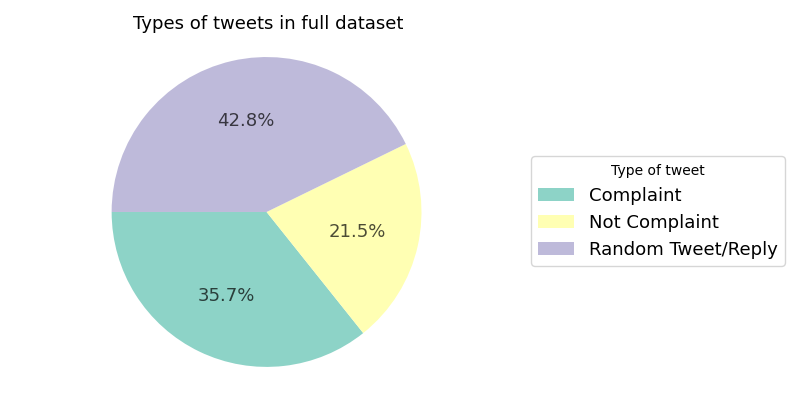
\includegraphics[width=9cm]{figures/compl_non_random_dist.png}
    \vspace*{-3mm}
    \caption{Illustrates the distribution of tweets categorised as 'complaints' and 'not complaints', with random 'tweets / replies' shown separately.}
    \label{fig: compl_non_random_dist}
\end{figure}


All tweets categorised as complaints are assigned the label \texttt{label:1}, while tweets that do not constitute complaints are assigned \texttt{label:0}. In terms of class distribution, the dataset is skewed towards 'not complaint' tweets, as depicted in Figure \ref{fig: compl_non_random_dist}, where \texttt{label:1} represents 35.7\% and \texttt{label:0} represents 64.3\% of the dataset. To ensure a more representative dataset, the authors of \cite{preotiuc-pietro_automatically_2019} introduced several random tweets and replies. This approach aligns with the real-world scenario where complaint-related posts form a smaller proportion within an organization's social media tweets and posts. Additionally, this strategy has the potential to enhance the model's ability to generalize effectively during the finetuning process.\\

\begin{figure}[htbp]
    \centering
    \captionsetup{font=small}
    \begin{subfigure}{0.49\textwidth}
        \centering
        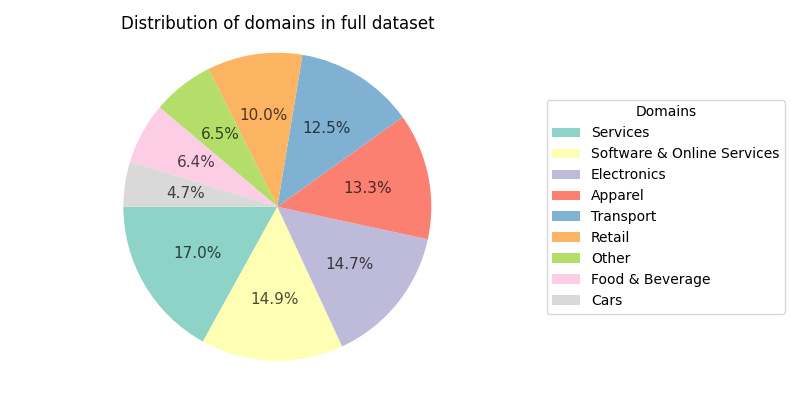
\includegraphics[width=\linewidth]{figures/domain_dist.png}
        \caption{Proportion of each domain}
        \label{fig: domain_dist_pct}
    \end{subfigure}
    \hfill
    \begin{subfigure}{0.49\textwidth}
        \centering
        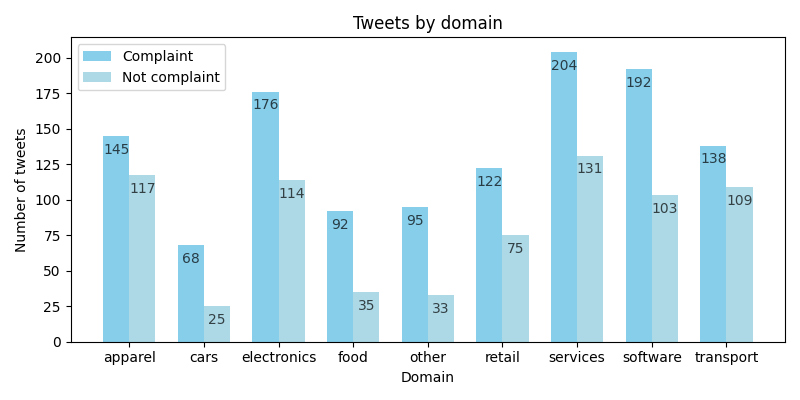
\includegraphics[width=\linewidth]{figures/domain_counts_bar_norandom.png}
        \caption{No. of tweets for each domain}
        \label{fig: domain_dist_count}
    \end{subfigure}
    \caption{Shows the distribution of the domains used in the dataset}
    \label{fig: compl_main_dist}
\end{figure}

The dataset comprises domains encompassing both complaint-related tweets and non-complaint tweets. Figure \ref{fig: domain_dist_pct} illustrates the distribution of domains, with the top 3 categories being services, software, and electronics, collectively constituting nearly 50\% of the tweets. A key observation from Figure \ref{fig: domain_dist_count} is the prevalent class imbalance within most domains, accompanied by relatively low tweet volumes within each domain. The implications of these observations on predictions are analyzed in Experiments set 2 and elaborated upon later in this chapter.

\begin{figure}[htbp]
    \centering
    \captionsetup{font=small}
    \begin{subfigure}{0.49\textwidth}
        \centering
        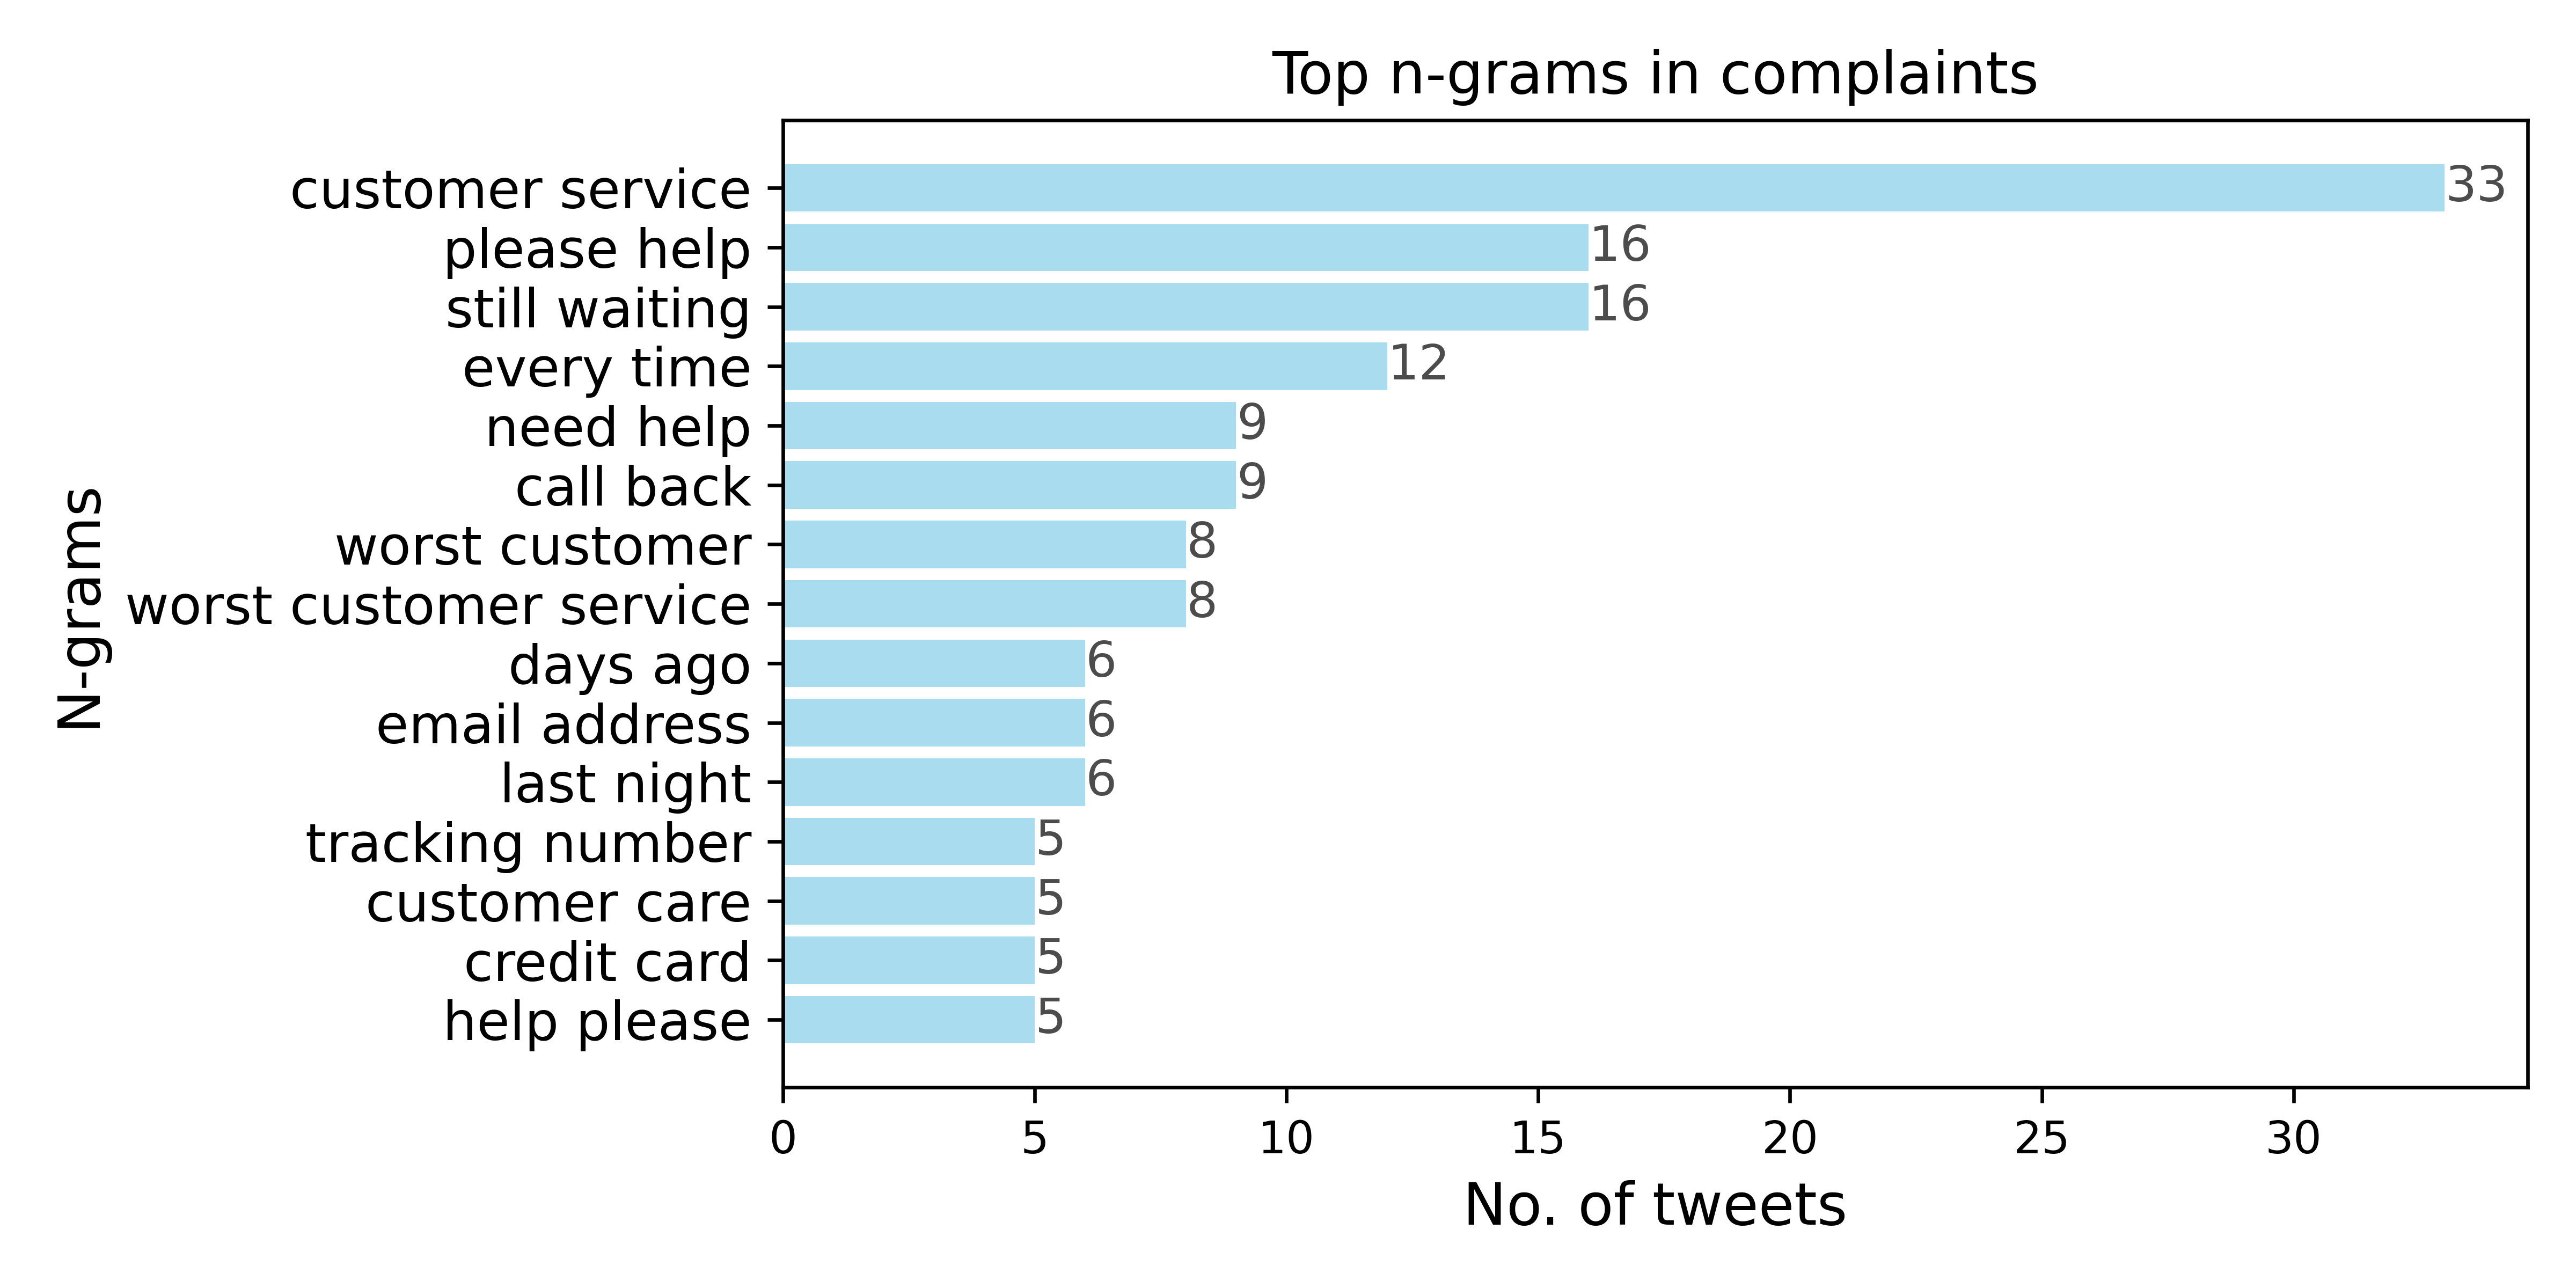
\includegraphics[width=\linewidth]{figures/top_ngram_horiz_bar.png}
        \caption{Top n-grams}
        \label{fig: top_ngrams}
    \end{subfigure}
    \hfill
    \begin{subfigure}{0.49\textwidth}
        \centering
        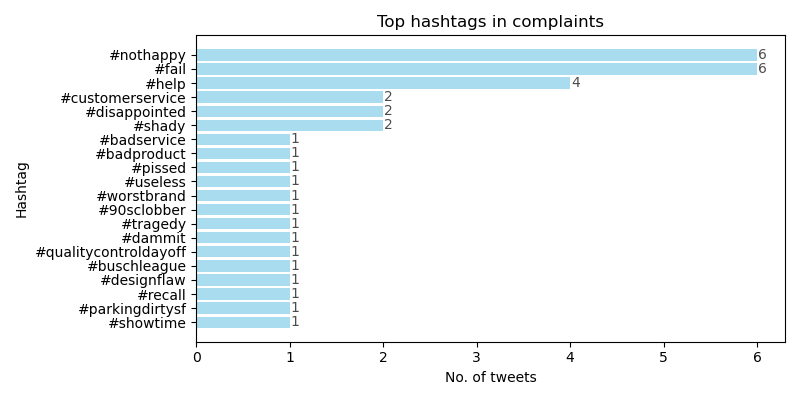
\includegraphics[width=\linewidth]{figures/top_hash_horiz_bar.png}
        \caption{Top hashtags}
        \label{fig: top_hashtags}
    \end{subfigure}
    \caption{Top n-grams(excl. unigrams) and hashtags in the complaint tweets.}
    \label{fig: top_ngrams_hashtags}
\end{figure}

Analysing further on the text used in complaints on Twitter, the most frequent n-grams as shown in Figure \ref{fig: top_ngrams} are terms involving an expectation of rectification (e.g. please help, need help), an expression of frustration (e.g. still waiting, worst customer service, call back) or other aspects related to general customer service (e.g. tracking number, customer care). This is in line with how a complaint is defined as described in the earlier chapters. There are also other characteristics touched upon earlier that are evident in the tweets, including varying levels of anger or frustration, altuirism (warning others),  \\

\textbf{Examples expectation of rectification}
\begin{itemize}
    \item[\textbullet]\textit{"hey chrysler cares i'm the one with the 2011 200 need help with the heating . inside the car it's really strange"}
    \item[\textbullet]\textit{"can someone please help me ? i've already sent a dm ."}
\end{itemize}
\textbf{Examples expression of frustration}
\begin{itemize}
    \item[\textbullet]\textit{"worst customer service experience with <user> <user> <user> . never been treated with such contempt"}
    \item[\textbullet]\textit{"on hold with <user> an hour just to get told to call back another day . hell yeah"}z
    \item[\textbullet]\textit{worst customer service to-date <user> in greensboro off wendover . avoid this place and let's show them we have other choices . \#otherchoices}
\end{itemize}


\begin{table}[htbp]
    \captionsetup{font=small}
    \centering
    \begin{tabularx}{\textwidth}{|X|c|c|c|c|}
        \hline
        \rowcolor[gray]{0.7}
        \textbf{Statistic}              & \textbf{All Tweets} & \textbf{Complaints} & \textbf{Not Complaints} & \textbf{Random} \\
        \hline
        Number of tweets                & 3,449               & 1,232               & 742                     & 1,475           \\
        \hline
        Number of unique tweets         & 3,395               & 1,232               & 737                     & 1427            \\
        \hline
        \hline
        Max tweet length (char.)        & 297                 & 297                 & 266                     & 144             \\
        \hline
        Min tweet length (char.)   .    & 1                   & 7                   & 6                       & 1               \\
        \hline
        Mean tweet length (char.)       & 77.8                & 96.7                & 70.2                    & 65.8            \\
        \hline
        Median tweet length (char.)     & 79.0                & 98.0                & 68.0                    & 63.0            \\
        \hline
        Standard Deviation tweet length & 41.4                & 40.5                & 38.9                    & 37.5            \\
        \hline
        \hline
        Total number of tokens          & 55,169              & 24,260              & 10,839                  & 20,070          \\
        \hline
        No. of unique tokens            & 7,937               & 4,031               & 2,558                   & 4,386           \\
        \hline
        Maximum tokens                  & 57                  & 57                  & 55                      & 39              \\
        \hline
        Minimum tokens                  & 1                   & 2                   & 1                       & 1               \\
        \hline
        Mean tokens                     & 16.0                & 19.7                & 14.6                    & 13.6            \\
        \hline
        Median tokens                   & 16.0                & 20.0                & 14.0                    & 13.0            \\
        \hline
        Standard Deviation for tokens   & 8.6                 & 8.4                 & 8.0                     & 8.0             \\
        \hline
        \hline
        Average punctuation count       & 3.4                 & 3.9                 & 2.7                     & 3.3             \\
        \hline
    \end{tabularx}
    \caption{Statistics of tweets in the dataset.}
    \label{tab: tweets_statistics}
\end{table}



\section{Comparision of model performance}
**TO UPDATE**

\section{Analysis of best performing model}
**TO UPDATE**

\section{Cross-domain results}
**TO UPDATE**